\section{Cor}

\begin{frame}[allowframebreaks]
  \frametitle{Cor}
  O CIE define cor como o resultado perceptivo de luz no espectro visível, com comprimento de onda
  entre 400 e 700nm, incidente na retina. 

  \begin{figure}[h!]
  \centering
  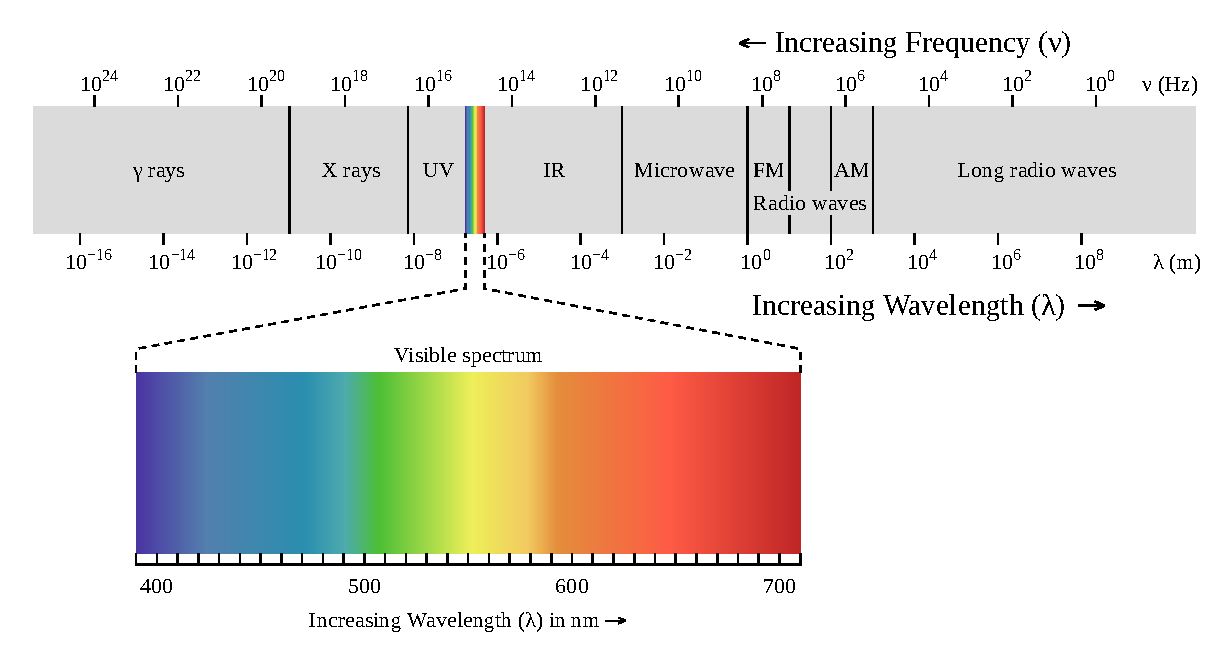
\includegraphics[width=0.6\textwidth]{images/emspectrum.pdf}
  \caption{Espectro Eletromagnético (Wikipedia).} 
  \label{fig:emspectrum}
  \end{figure}
 
  \framebreak

  Espectro das cores e o metamerismo.

  \begin{columns}[T]
  \column{.33\textwidth}  
    \begin{figure}[h!]
    \centering
    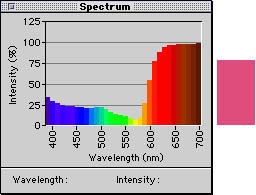
\includegraphics[width=0.8\textwidth]{images/spd_red.jpg}
    \caption{Espectro do vermelho oxicoco (\textit{cranberry}) (\hrefcolor{https://creativepro.com/out-of-gamut-why-is-color/}{Bruce Fraser})}
    \label{fig:spd_red}
    \end{figure}
  \column{.33\textwidth}
    \begin{figure}[h!]
    \centering
    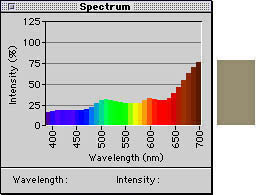
\includegraphics[width=0.8\textwidth]{images/spd_green1.jpg}
    \caption{Espectro do verde. Exemplo de Metamerismo. (\hrefcolor{https://creativepro.com/out-of-gamut-why-is-color/}{Bruce Fraser})}
    \label{fig:spd_green1}
    \end{figure}
  \column{.33\textwidth}
    \begin{figure}[h!]
    \centering
    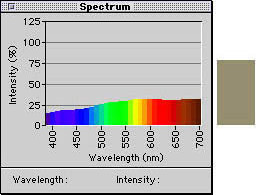
\includegraphics[width=0.8\textwidth]{images/spd_green2.jpg}
    \caption{Espectro do verde. Exemplo de Metamerismo. (\hrefcolor{https://creativepro.com/out-of-gamut-why-is-color/}{Bruce Fraser})}
    \label{fig:spd_green2}
    \end{figure}
  \end{columns}

  \framebreak

  \begin{figure}[h!]
  \centering
  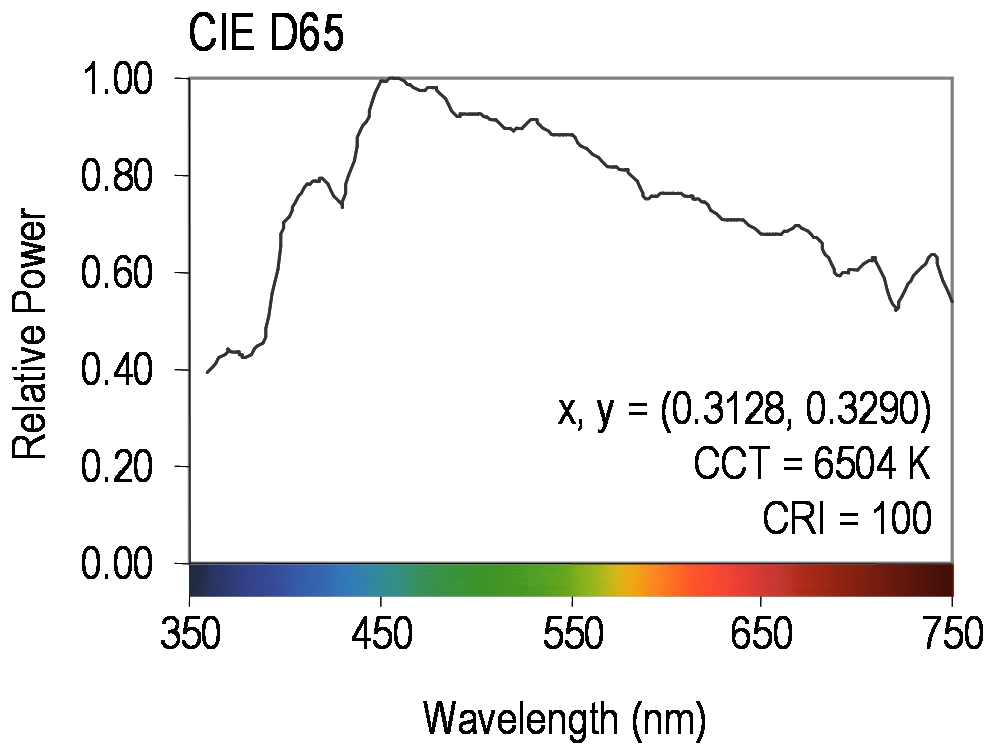
\includegraphics[width=0.5\textwidth]{images/D65.png}
  \caption{Distribuição espectral de potência do D65 (Wikipedia).}
  \label{fig:D65}
  \end{figure}
\end{frame}
\note{
Metametismo é quando duas ou mais cores possuem composições espectrais distintas, mas aparentam possuir a mesma cor.

\url{https://en.wikipedia.org/wiki/Metamerism_(color)}
}
\note{
A cor percebida de um objeto depende das suas características de absorção-reflexão e também das características da luz incidente.

\vspace{3ex}
O padrão D65 do CIE refere-se à característica espectral do iluminante, correspondendo 
à iluminação solar ao meio-dia na Europa ocidental, composta pela luz direta e difundida em céu limpo.

\url{https://en.wikipedia.org/wiki/Color_temperature}
}



\begin{frame}[allowframebreaks]
  \frametitle{Espaços de Cores}
  As cores podem ser organizadas em diferentes espaços. O espaço de cor, juntamente com as 
  características do dispositivo definem a extensão de cores que poderão ser representadas.

  Alguns espaços de cores:
  \begin{itemize}
  \item RGB 
  \item CMYK
  \item YUV
  \item YCbCr
  \item CIELAB
  \end{itemize}

  \url{https://en.wikipedia.org/wiki/Color_space}

  \framebreak
  \textbf{YCbCr}

  Y' é a componente de luma
  
  Cb e Cr são componentes de crominância, diferença de azul e diferença de vermelhor, respectivamente
  
  \begin{equation}
  \begin{aligned}
   Y' &= K_R \cdot R' + (1 - K_R - K_B) \cdot G' + K_B \cdot B'\\
   P_B &= \frac12 \cdot \frac{B' - Y'}{1 - K_B}\\
   P_R &= \frac12 \cdot \frac{R' - Y'}{1 - K_R}
  \end{aligned} \nonumber
  \end{equation}
  convenção ITU-R BT.601: \\
  $K_B = 0.114$ e $K_R = 0.229$.


  \framebreak
  \textbf{JPEG}

  \begin{equation}
  \begin{aligned}
   Y'  &=&     &+ (0.299    \cdot& R'_D) &+ (0.587    \cdot& G'_D) &+ (0.114    \cdot& B'_D) \\
   C_B &=& 128 &- (0.168736 \cdot& R'_D) &- (0.331264 \cdot& G'_D) &+ (0.5      \cdot& B'_D) \\
   C_R &=& 128 &+ (0.5      \cdot& R'_D) &- (0.418688 \cdot& G'_D) &- (0.081312 \cdot& B'_D) 
  \end{aligned} \nonumber
  \end{equation}
  
  \begin{equation}
  \begin{aligned}
  R  &=& Y                            &&& + 1.402   \cdot &(C_R-128) \\
  G  &=& Y   &- 0.34414 \cdot &(C_B-128)& - 0.71414 \cdot &(C_R-128) \\
  B  &=& Y   &+ 1.772   \cdot &(C_B-128)&
  \end{aligned} \nonumber
  \end{equation}

\end{frame}

\begin{frame}[allowframebreaks]
  \frametitle{Correção Gamma}

  A correção gamma é definida pela seguinte expressão:
  \begin{equation}
  V_{\text{out}} = A {V_{\text{in}}}^{\gamma} \nonumber
  \end{equation}
  onde $A$ é uma constante e os valores de entrada são valores reais não negativos 
  (tipicamente normalizados entre 0 e 1).

  \begin{figure}[h!]
  \centering
  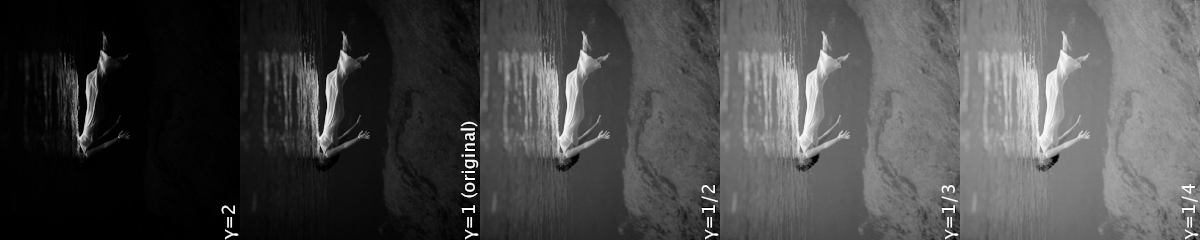
\includegraphics[width=0.9\textwidth]{images/gammacorrection.jpg}
  \caption{Correção gamma (Wikipedia).}
  \label{fig:gammacorrection}
  \end{figure}
  
\end{frame} 
\note{
``Gamma encoding of images is used to optimize the usage of bits when encoding an image (...)
The human perception of brightness (lightness), under common illumination conditions (neither pitch black nor blindingly bright), follows an approximate power function (note: no relation to the gamma function), with greater sensitivity to relative differences between darker tones than between lighter tones, consistent with the Stevens power law for brightness perception. If images are not gamma-encoded, they allocate too many bits or too much bandwidth to highlights that humans cannot differentiate, and too few bits or too little bandwidth to shadow values that humans are sensitive to and would require more bits/bandwidth to maintain the same visual quality.
''

\url{https://en.wikipedia.org/wiki/Gamma_correction}
}
